\chapter{Gaze-independent visual \acsp{bci}}
\label{sec:gaze-independent}
\epigraph{%
  ``\elide\ This begs the question: if a patient had reliable control
  over their eye gaze, why would one aim to facilitate communication with that
  patient via a BCI? It would be far simpler and more efficient to use an
  eye-tracking system.
  And even if a BCI were the preferred or only available option for some reason,
  designs requiring eye gaze control could not be used
  by patients with severe motor impairment, as these patients
  cannot direct their gaze.
  Because these are the patients who have the greatest need for BCIs, it is
  important that accurate gaze-independent BCIs exist.''
}{%
  \textcite{Egan2017}
}

\noindent\emph{The last paragraph of \cref{sec:gaze-independence/sota},
\cref{sec:gaze-independence/oculomotor/gaze}, and the first paragraph of
\cref{sec:gaze-independence/objectives} were adapted from
\textcite{VanDenKerchove2024}.}

\section{Eye motor impairment in individuals with \acl{sspi}}%
\label{sec:gaze-dependence}

One of the goals of brain-computer interfacing is establishing a communication
channel that does not rely on speech or muscular activity, which in turn can
provide solutions to individuals with \ac{sspi}.
In the strictest interpretation, this means that an interface should not
rely on the control of eye muscles used to redirect the gaze or for blinking.
It is exactly this potential of \acp{bci} that makes them suitable as assistive
communication devices.

\subsection{Incidence of eye motor impairment}
\label{sec:gaze-independent/gaze-dependence/incidence}
\Ac{sspi} is often caused by damage to the central or peripheral nervous
system, either through congenital diseases (\ac{cp}, \ac{fa}, \ldots),
neurodegenerative (\ac{als}, \ac{ms}, \ldots) or acquired (stroke and
\ac{tbi}).
Many individuals in these groups are unfortunately also afflicted by some form
of eye motor impairment, requiring \acp{bci} adapted to their condition.
\Cref{tab:incidence} reports the relatively high frequencies of
eye motor impairment, which can range from minor (nystagmus,
\footnote{Involuntary, rhythmic, and repetitive eye movements recognizable by their
consistent directionality (horizontal, vertical, or rotational).},
other eye tremors
\footnote{These can include square-wave jerks, saccadic intrusions, microtremors, or
microsaccades while resting or fixating the gaze.},
gaze fixation fatigue or discomfort, \ldots), to severe (partial ophthalmoplegia
\footnote{Weakness or limited paralysis of one or more of the muscles that control eye
movement, leading to restricted eye motion, but not complete paralysis.
Often, a specific movement direction (up-down, left-right) is preserved.},
involuntary movements, impaired pursuit, \ldots), and even complete
ophthalmoplegia\footnote{Full eye movement paralysis.} or eye motor paresis.
This not only affects vision and coordination but also
their ability to operate a visual \ac{bci}~\cite{FriedOken2020}.

\begin{table}
  \centering
  \makebox[\textwidth][c]{%
  \small
\sffamily
\begin{tabularx}{\textwidth}{@{}Xccccccccc@{}}
\toprule
    & \bfseries \acs{als} & \bfseries \acs{ms}   & \bfseries Stroke
    & \bfseries \acs{cp} & \bfseries\acs{fa} & \bfseries \acs{dmd} & \bfseries \acs{sma} & \bfseries \acs{lis} \\ \midrule
    \bfseries Minor    & 50\% & 31\% & 40-70\% & + & 100\% & + & - &      \\
    \bfseries Severe   & 33\% & 3\%  & +       & 60-100\% & >5\% &  - & - & 98\% \\
    \bfseries Complete & 17\%\footnote{In late-stage \ac{als}.} & -    & +
    & -&- & - & - & 2\%  \\
\bottomrule
\end{tabularx}

  }
  \caption[Incidence of eye motor impairment in selected \acs{bci} user target
    populations.]{%
      Incidence of eye motor impairment in selected \ac{bci} user target
      populations. \acs{als}: \acl{als}, \acs{ms}: \acl{ms}, \acs{dmd}:
      \acl{dmd}, \acs{sma}: \acl{sma}, \acs{cp}: \acl{cp}, \acs{lis}: \acl{lis}.
      $+$: frequent, $-$: infrequent.
    }
    \label{tab:incidence}
\end{table}

Among the most affected are those recovering from stroke~\cite{Pollock2011,Rowe2019},
and most of all those with due to brainstem or cerebellar stroke~\cite{Moncayo2009,Bogousslavsky1987}.
Stroke can lead to the most severe severe or even complete eye motor impairment
from the onset of their condition, resulting in the~\ac{lis}.
However, case study reports~\cite{Patterson1986,Graber2016} show that even in individuals
with \ac{lis} due to stroke, the group with a complete lack of eye motor
control is very small.

\ac{als} is progressive disease affecting motor neurons.
This initially results in general weakness and loss of muscle tone, but
eventually leads to full body paralysis.
Although eye movement is often cited as one of the longest preserved
capabilities in \ac{als}, studies show that minor issues are still
fairly common~\cite{Kang2018, Guo2022,Moss2012}.
The bulbar-onset variant is characterized by an early loss of speech
and increased involvement of eye motor symptoms~\cite{Guo2022}.
Furthermore, \textcite{Hayashi1991} show that as \ac{als} progresses past
the point of independent breathing, symptoms will eventually also involve
eye muscle paralysis.
One of the goals of \ac{bci} has always been to support these individuals to
ensure quality of life.

Various forms of eye movement abnormalities also occur often in
\ac{ms}.
\Ac{ms} is a neurodegenerative disease involving demyelination of nerves.
Eye motor abnormalities are especially well
studied~\cite{Mueri1985,Prasad2010,Castelnovo2016,Serra2018,Polet2020} and
are often used as diagnostic tools.
These abnormalities can be minor or severe, seldom progressing to complete
paralysis.
However, \ac{ms} often comes with vision loss, further complicating interaction
with visual \acp{bci}.

\Ac{fa} is a neurodegenerative disease affecting the
spinal cord, peripheral nervous system, and cerebellum, resulting in an
impairing loss of muscle coordination.
This almost always heavily affects eye
movements~\cite{Fahey2008,Hocking2010,Furman1983,Cook2017}, with various forms of
involuntary movements and trouble pursuing or fixating on targets.
They also gradually have more trouble speaking but often retain some muscular
control.

Another other group that is heavily affected, is \ac{cp}~\cite{Fazzi2012}.
Additionally, individuals with other neurodegenerative diseases like
\ac{sma}~\cite{Anagnostou2021} and \ac{dmd}~\cite{Lui2001} are
sometimes also interested in \ac{bci} use, but their eye motor capabilities are
mostly preserved.

\subsection{Gaze impairment and \acl{lis}}
\label{sec:gaze-independence/oculomotor/gaze}
\newcommand\fnlis{\footnote{Multiple definitions of \ac{lis} are encountered in
\ac{bci} and neurological literature.
Some definitions include only those with tetraplegy without eye movements used
for communications.
Others distinguish Complete Locked-in Syndrome (CLIS) with full body paralysis,
including no eye motor control at all, from a \ac{lis} state with some preserved eye
movements or minor motor output.
While some definitions only include stroke or \ac{tbi} with damage to
specific regions in the brain (midbrain, brainstem, or
cerebellum)~\cite{Smith2005}, it can also generally refer to the state of full body paralysis
or loss of muscle tone incurred in neurodegenerative diseases, combined with
the inability to speak, such as occurs in late-stage ALS.}}

\newcommand\fnwolpawcrit{\footnote{
``The first class consists of people who are truly totally locked-in (e.g.,
due to end-stage ALS or severe cerebral palsy), who have no remaining
useful neuromuscular control of any sort, including no eye movement.
\elide\ This class is very small. \elide\
The second class of potential \ac{bci} users comprises those who retain
a very limited capacity for neuromuscular control. This group includes
people who retain some useful eye movement or enough limb muscle
function to operate a single-switch system. Such control is often slow,
unreliable, or easily fatigued.
This group is much larger than the first.''~\cite{Wolpaw2006}}}

We believe it is generally not opportune to delve too deeply into the underlying
ophthalmological and neurological mechanisms for each of the specific
conditions, or even the exact symptoms.
In clinical reality, every \ac{bci} user has different symptoms, which lead to their own
unique set of preserved capabilities and visual skills.
From a solution-oriented \ac{bci} engineering point of view, the etiology of the symptoms can be abstracted away.
Instead of categorizing users by their etiology, we will refer to those who might benefit from
\ac{bci} assistive communication technology as having \ac{sspi}, in line with
the terminology used by~\textcite{FriedOken2020}.
If they have eye motor impairment that affects their use of visual \ac{bci} or
eye-tracking solutions, we use the term \ac{sspgi} (see \cref{fig:gaze-independence/venn}).

\begin{figure}
  \sffamily
\begin{tikzpicture}

    % Draw the outer lightgray box with ultra thick darkgray line
    \draw[fill=lightgray, draw=darkgray, ultra thick] (-4,-1.5) rectangle (4,5.5);
    % Label for the outer box in the top left corner
    \node[anchor=north west, text=darkgray] at (-4,5.5) {\textbf{\acs{bci} users}};

    % Draw the outermost circle for SSPI with ultra thick lines and bold text matching its line color
    \draw[ultra thick, accent1] (0,2) circle (3);
    \node[text=accent1] at (0,4) {\textbf{\acs{sspi}}};  % Centered bold text with line color

    % Draw the middle circle for SSPGI with ultra thick lines and bold text matching its line color
    \draw[ultra thick, accent2] (0,1) circle (2);
    \node[text=accent2] at (0,1.66) {\textbf{\acs{sspgi}}};  % Centered bold text with line color

    % Draw the innermost circle for LIS with ultra thick lines and bold text matching its line color
    \draw[ultra thick, accent3] (0,0) circle (1);
    \node[text=accent3] at (0,0) {\textbf{\acs{lis}}};  % Centered bold text with line color

\end{tikzpicture}

  \caption[Venn diagram of potential users of \acs{bci} assistive technology.]{%
    Venn diagram of potential users of assistive technology.
    Patients with \acf{sspi} are the general target population.
    If eye gaze-based solutions are not properly suited for an individual,
    they have \acf{sspgi}.
    Individuals with \ac{lis} have no muscular control left, or it is very limited,
    such as the ability to communicate through a binary switching system.
    \Acp{bci} are especially relevant for the last two groups, as they are not
    able to use eye tracking solutions.
  }
  \label{fig:gaze-independence/venn}
\end{figure}

The most severely impaired of the user groups above constitute the \ac{lis}
group, which forms one of the main \ac{bci} interest groups.
In this work, we use the term \ac{lis} for a situation of (near)
complete paralysis and difficulties or the inability to communicate independently,
even with assistive technology.
This corresponds to classes one and two defined by
\textcite{Wolpaw2006}\fnwolpawcrit.
Hence, some degree of severe or complete eye motor impairment is usually
necessary to qualify as locked-in\fnlis.

In general, the group of locked-in individuals with complete loss of eye motor
function is very small.
Hence, it would be interesting to focus \ac{bci} development efforts on the
larger population of individuals with \ac{sspgi} who currently slip through
the cracks of the assistive technology offerings.
These are individuals whose severe eye motor impairment prevents them from
using eye-tracking-based solutions.
They currently use their remaining motor control to
communicate by indicating symbols on a letterboard with great effort,
or signal with upward eye movements or blinks to confirm prompted letters.
They require a caregiver or relative to interpret their signals and crave
the ability to communicate independently, which is crucial to retaining an
acceptable quality of life.

This brings us back to the gaze-dependence problem in visual \ac{bci}:
Traditional visual \ac{bci} scenarios require the user to \emph{overtly} direct both their
\ac{vsa} and gaze toward the screen target they intend to select.
However, a critical challenge arises when users rely solely or in part on
\emph{covert} \ac{vsa}, which involves directing \ac{vsa} without corresponding
eye gaze.
In these cases, classical solutions often fall short of the widely accepted
80\% target selection accuracy threshold~\cite{Brunner2010,Frenzel2011,Treder2010,RonAngevin2019}
deemed necessary for a comfortable user experience~\cite{Neeling2019}, calling for alternative, gaze-independent
solutions.

In this work, we will use the term \emph{gaze-independent} to mean
\emph{`dealing explicitly with the fact that a user cannot control their
gaze.'}
In the context of a visual \ac{bci}, this means that the user's
visuospatial attention and their gaze do not necessarily coincide.
There are multiple approaches to implement gaze-independence in a \ac{bci}.
The next section highlights some noteworthy examples.

\section{State-of-the-art}
\label{sec:gaze-independence/sota}

\subsection{Gaze-independent modalities}
Gaze-independent \ac{erp}-based \acp{bci}~\cite{Riccio2012, Aloise2012} can be realized in three
ways.
Firstly, active \ac{bci} communication paradigms relying on endogenous activation from the user
do not rely on sensory stimulation.
Examples of this are imagined movement or imagined speech paradigms.
These paradigms can yield very high information transfer
rates~\cite{Willett2021,Metzger2023}, both due to their intuitiveness and the
complexity that can be captured in commands, but they often do so only when paired
with invasive recording.
Non-visual reactive paradigms that use, for example, auditory~\cite{Halder2010} and
somatosensory~\cite{Brouwer2010}
stimulation do not rely on gaze redirection but also result in lower \acp{itr}
compared to visual paradigms, with \acp{itr} ranging between 1 and 10 bits/min
for auditory paradigms and 0.5 and 5 bits/min for tactile~\cite{Riccio2012}.
While auditory and somatosensory stimulation on their own might yield poor
\ac{itr}, \textcite{Yin2016} showed that it can provide added value in gaze-independent
settings when coupled with oddball stimulation in a hybrid paradigm.
Their solution using the P3 components of bimodal stimulation reached an \ac{itr} of 14.94 bits/min.
In general, their approach is interesting as it follows a philosophy that
relies on establishing as many communication pathways as possible.
Yet, auditory and somatosensory \acp{bci} suffer from increased mental effort in
operation and from user-dependent
variability~\cite{Severens2014,Reichert2020b}.
\textcite{Severens2014} showed that the visual Hex-o-Spell~\cite{Treder2010}
outperformed a somatosensory alternative in participants with \ac{als} whose
eye motor capabilities were effectively impaired.

\subsection{Gaze-independent visual stimulation}
\label{sec:gaze-independence/sota/visual}

This leads us to the second approach: current visual stimulation paradigms can be optimized so that
the stimuli are always present in the field of view, either overtly~\cite{Acqualagna2013, Won2018, Lin2018} or covertly~\cite{Pires2011,Lees2018}.
Some noteworthy examples include the GIBS Block Speller~\parencite{Pires2011},
the GeoSpell interface~\parencite{Aloise2012}, and the \ac{rsvp}
speller~\parencite{Acqualagna2011}.
The \ac{rsvp} paradigm, in particular, is a prime contender for a performant gaze-independent
\ac{bci}.
\textcite{Lin2018} reported an average online \ac{itr} of 20.259 bits/min using
a paradigm with subsequently flashing sets of three characters filling the user's field of view.
We make a distinction here between spatially organized interfaces, where
multiple targets are displayed at the same time at different spatial locations,
and temporally organized interfaces, like \ac{rsvp}, where targets or small
sets of targets (e.g. 3) are shown consecutively.
The Hex-o-Spell, GeoSpell, and GIBS Block Speller are spatially organized, while
variants of the \ac{rsvp} paradigm are temporally organized.
\textcite{Lin2018} follow the philosophy that spatially organized interfaces
have historically not performed well in the presence of gaze impairment.
However, we argue that spatially organized interfaces generally have a much higher
\ac{itr} in healthy controls.
For instance, a regular matrix-based speller can achieve an \ac{itr} of up to
30 bits/min.
With the right set of adaptations, spatial attention could potentially also
bring added value to individuals with \ac{sspgi}.
While spatial interfaces are indeed more gaze-dependent than temporal
interfaces, they also provide an extra channel that can be used to transfer
information, i.e., the location of the stimulus.

As an alternative to spatial attention, non-spatial visual attention (feature attention) can also be exploited, such as
attention to stimulus color, shape, or symbol~\cite{Zhang2010,Treder2011,Hwang2015}.
The \ac{rsvp} speller is already an example of this, relying on the user to
attend to the appearance of the intended character to type.
Visual stimulation paradigms relying on alternative types of attention
can modulate specific extra \ac{erp} components that either improve performance
because they embed extra information in the brain signal~\cite{Xu2022}
or because they are more sensitive to stimulation in the visual
periphery~\cite{Schaeff2012}.
Nevertheless, solely relying on alternative types of attention can also suffer from
reduced information transfer rates~\cite{Chennu2013}.
Furthermore, the previously mentioned systems were typically tested only in
settings where the user was required to focus on a central fixation point while
selecting peripheral targets.
This entails that they still rely to some extent on
eye motor control, often necessitating central gaze fixation.

\subsection{Gaze-independent decoding}
\label{sec:gaze-independence/sota/decoding}

Thirdly, stimuli can be presented in a standard \ac{bci} paradigm, but visuospatial
attention can be decoded separately from gaze direction.
\textcite{Aloise2012} aimed to bridge the performance gap between covert and
overt \ac{vsa} decoding performance.
They compared classical linear and non-linear \ac{erp} classifiers on a covert
attention oddball \ac{erp} paradigm dataset.
The results revealed no significant performance improvement in covert \ac{vsa}
decoding for any of the investigated decoders.

More recent work has made advances in decoding lateralized covert
\ac{vsa} by harnessing the N2pc \ac{erp}
component~\cite{Thiery2016,Reichert2020b,Wang2022}.
The amplitude of the N2pc component in the contralateral hemisphere is directly modulated
by the location of covert \ac{vsa}.
Another approach is directly decoding covert shifts in \ac{vsa} from spectral
content~\cite{Tonin2013}.
These methods are promising, but to date often require a slower stimulation pace or cannot display as
many targets as the classical \ac{erp} \ac{bci} paradigms.
As with the alternative modality approach, they are currently only helpful as
extra communication channels in a hybrid paradigm.
\textcite{Xu2016} reached an \ac{itr} of 23.56 bits/min by detecting the N2pc
component while performing \ac{ssvep} stimulation.
\textcite{Egan2017} also showed an increase in \ac{ssvep} performance by
concurrently decoding the covert \ac{vsa} shift from spectral content, but
their study only used two stimulation targets.
In general, we conclude that gaze-independent decoding in the fast-paced reactive
\ac{erp} paradigm leveraging spatial attention remains underexplored.

\section{Research objectives}
\label{sec:gaze-independence/objectives}

To summarize, for individuals with \ac{sspgi}, gazing directly at a screen target may
be uncomfortable, impractical, or even impossible.
Hence, assistive devices that rely on eye tracking are often inefficient for
them.
Consequently, while \acp{bci} hold great promise for these individuals, conventional
gaze-dependent \ac{bci} solutions do not meet their needs due to the absence of gaze
control.
Therefore, the development of decoding strategies that account for covert
\ac{vsa} becomes crucial in the pursuit of high-performance gaze-independent
\acp{bci}.

The general goal of this PhD is to tackle the gaze-dependence problem in the
visual oddball \ac{bci}.
\Cref{sec:gaze-independence/sota} showed that visual \ac{bci} paradigms are a
good candidate for a performant gaze-independent \ac{bci}.
While the central gaze fixation of most visual gaze-independent paradigms still
relies to some extent on eye motor control, we aim to circumvent this.
In such an interface, stimuli can be presented in a standard \ac{bci} paradigm, but
visuospatial attention can be decoded separately from gaze position, which do not necessarily need to coincide.

This leads us to adopt a specific approach: \emph{improve the performance of a
spatially organized visual oddball \ac{erp}-based brain
computer interface by using a suited decoding strategy}.

To achieve our goal, we chose a suitable interface and innovate on decoder
development.
We collect data from healthy control subjects to test our decoders.
Finally, the findings of these experiments will be verified in experiments with
individuals with \ac{sspgi}, including individuals with \ac{lis}, evaluating
both performance and comfort.

This specific target is embedded within a broader goal of enabling
effective communication for those with \ac{sspgi}.
Ultimately, we wish to design a comfortable interface that allows them to maximally exploit
their residual gaze capabilities.
We believe this can be done with a non-invasive, spatially
organized visual \acp{bci} with high \ac{itr}.
Finally, our efforts also aim to improve \ac{erp} decoding performance
in general, which will also contribute to their effectiveness in both gaze-dependent
and gaze-independent settings.


\section{Approach}

\subsection{Decoder design}

During this PhD, we explored different lines of decoding strategies,
trying to tackle several challenges, be they general problems in \ac{erp} decoding
or those that arise specifically from gaze-independence.
Examples of these challenges include the lack or decrease in the amplitude of specific \ac{erp} components, and the increased
non-stationarity of the signal.
As mentioned, state-of-the-art decoders have poor performance in covert attention
settings.
The general goal is thus to design a machine learning classifier that represents
the \ac{erp} signal in a way that makes it more robust to the problems
occurring in covert attention conditions.

\subsubsection{Regularized spatiotemporal beamforming}

Due to the decreased amplitude of the N1 and P3 components in covert attention
settings~\cite{Treder2010}, the \ac{snr} of
the \ac{erp} is lower than in overt attention settings.
Therefore, a straightforward way to reach satisfactory
gaze-independent decoding performance may be to increase overall \ac{erp}
decoding performance.

To address this, we improved upon an in-house developed, state-of-the-art \ac{erp}
decoder, the \ac{stbf}~\cite{Wittevrongel2016}, by reformulating
this classifier as a linear discrimination problem and
imposing regularizing constraints by structuring the noise covariance matrix
(\acs{stbf-struct}).
Furthermore, these regularizing constraints impose temporal stationarity on
the background noise, yielding insights for our next
efforts to cope with the non-stationarity of the P3 signal component.
This approach has been published by~\textcite{VanDenKerchove2022} and will be
described in \cref{sec:stbf-struct}.

\subsubsection{Tensor discriminant analysis}

In the context of \ac{bci} decoding, extracting robust and discriminative
features from multidimensional neural data is critical.
Tensor decoding methods offer a powerful approach by preserving the multiway structure
of \ac{eeg} data while optimizing class separability.
Unlike traditional methods that flatten data, TDA operates directly on tensors,
making it particularly suited for \ac{bci} applications, where signals are structured
across multiple channels and time points.

A widely used method is \ac{hoda}~\cite{Phan2010}, which projects tensors onto subspaces
optimized for class separation, similar to \ac{lda} but extended to multidimensional data.
This method has been applied to various \ac{bci} tasks, including \ac{erp} and
\ac{mi} decoding, enabling the extraction of class-relevant features while reducing
the data's dimensionality.

While \ac{hoda} is effective, it is limited by its reliance on a rigid core
structure, which may not fully capture the complexity of neural data in some
scenarios. To address this, \ac{bttda}
introduces a more flexible block-term structure.
\ac{bttda} iteratively extracts multiple blocks of
discriminative information, which can help in capturing more complex patterns
in neural data.
While \ac{bttda} is not specifically tailored to
gaze-independent \ac{bci} decoding, specific tensorizations of neural data can
offer advantages in coping with several obstacles arising from
gaze-independence.
The proposed \ac{bttda} method will be discussed in \cref{sec:bttda}.

\subsubsection{Classifier-based Latency Estimation with Woody iterations}

The previous two methods did not yet yield specific results in gaze-independent
decoding.
The following approach is targeted at improving decoding performance in
gaze-independent settings by accounting for a known property of the covert
attention \ac{erp} response.

P3 latency generally falls between 350ms and 600ms~\cite{Luck2014}, but this
value is heavily dependent on the subject and the task and can vary from trial
to trial~\cite{Ouyang2017}.
The work of \cite{Arico2014} illustrates that the variation in single-trial P3
latencies is important in gaze-independent decoding and has been hampering covert
\ac{vsa} decoding performance.
We reprised their hypothesis, stating that jitter compensation through latency
estimation and alignment improves
covert \ac{vsa} performance and extended it by developing a decoder.

Existing latency estimation methods are either not applicable to the
classification problem of labeling unseen data, or are not robust enough to
deal with the low \ac{snr} of the \ac{erp}.
\Ac{cble}~\cite{Mowla2017} is a technique that can leverage
\ac{erp} latency estimation in a decoding setting, but our results show that it
yields no improvement in gaze-independent settings.
We improved upon this technique and extended it to a probabilistic, iterative
method named \ac{wcble}.
This approach has been published by~\textcite{VanDenKerchove2024} and is presented
and evaluated on simulated data in \cref{sec:wcble}.
We have also collected datasets to evaluate this approach on real \ac{erp} data
in gaze-independent settings.

\subsection{Data collection}

\subsubsection{The CVSA-ERP dataset}
\label{sec:gaze-independence/approach/cvsa-erp}

In the first series of experiments, we recorded data using this interface from healthy participants.
The goal of these experiments was to benchmark
gaze-independent \ac{erp} decoding algorithms.
We denote this dataset as the Covert Visuospatial Attention \ac{erp} dataset
(CVSA-\ac{erp}).
This study was approved by the Ethics Commission of University Hospital Leuven
(S62547).
To simulate the dissociation between the eye gaze and the
intended target (\ac{vsa}), which could occur in individuals with gaze
impairment, healthy participants were cued to operate the \ac{bci} in specific
\ac{vsa} conditions.

We chose a visual oddball interface to study and adapt
to the effects of eye motor impairment on the \ac{erp}, using both existing state-of-the-art
decoders and our own proposed decoders.
Using a hexagonal layout interface, similar to the visual Hex-o-Spell proposed by
\textcite{Treder2010}, we presented six flashing circular targets
(without letters or symbols) to the participant while the EEG and
electro-oculogram (EOG) were recorded, along with eye gaze using eye tracking.
The Hex-o-Spell was chosen since it is optimized for gaze-independent
performance and because it has already been tested in individuals with
\ac{sspi} by~\textcite{Severens2014}.

The interface can be operated in different \ac{vsa} conditions, as illustrated in
\cref{fig:gaze/vsa}.

\begin{figure}
  \begin{subfigure}[t]{.45\textwidth}
    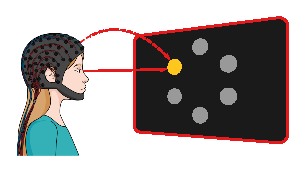
\includegraphics[width=\textwidth]{figures/gaze_independence/attention_overt.eps}
    \caption[Overt \ac{vsa}]{%
      \emph{Overt} \ac{vsa}.
      Gaze and \ac{vsa} coincide on a target.
    }
    \label{fig:gaze/vsa/overt}
  \end{subfigure}\hfill%
  \begin{subfigure}[t]{.45\textwidth}
    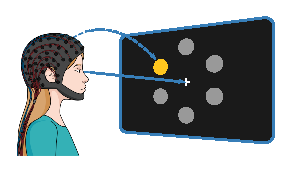
\includegraphics[width=\textwidth]{figures/gaze_independence/attention_covert.eps}
    \caption[Covert \ac{vsa}]{%
      \emph{Covert} \ac{vsa}.
      Gaze rests on the center of the screen, while \ac{vsa} is directed towards a target.
    }
    \label{fig:gaze/vsa/covert}
  \end{subfigure}

  \begin{subfigure}[t]{.45\textwidth}
    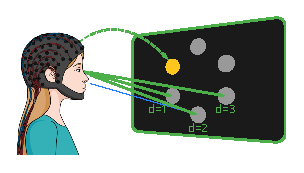
\includegraphics[width=\textwidth]{figures/gaze_independence/attention_split.eps}
    \caption[Split \ac{vsa}]{%
      \emph{Split} \ac{vsa}.
      \Ac{vsa} is directed towards a target, while the gaze rests on another.
    }
    \label{fig:gaze/vsa/split}
  \end{subfigure}\hfill%
   \begin{subfigure}[t]{.45\textwidth}
    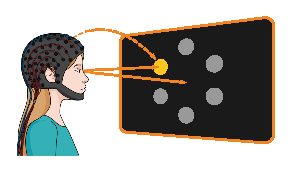
\includegraphics[width=\textwidth]{figures/gaze_independence/attention_free.eps}
    \caption[Free \ac{vsa}]{%
      \emph{Free} \ac{vsa}.
      The user is free to direct their gaze as they deem most comfortable.
      All previous \ac{vsa} conditions are possible.
    }
    \label{fig:gaze/vsa/free}
  \end{subfigure}\hfill%
  \caption[\Ac{vsa} conditions]{%
    \Acl{vsa} conditions defined in our hexagonal spatial \ac{erp} paradigm interface.
  }
  \label{fig:gaze/vsa}
\end{figure}

In the overt case, users gazed at the cued
target they were also mentally attending; in the covert case, users
gazed at the center of the screen while mentally attending to the cued target.
We introduced a \ac{vsa} condition that is understudied in the context of
gaze-independent \ac{bci} development: split \ac{vsa}.
In split \ac{vsa}, the user mentally focuses on one cued target while gazing at
another (the distractor).
This last option has been scarcely studied but completes
the options to dissociate gaze and visuospatial attention, allowing us to
investigate the effect of (the lack of) gaze control on \ac{bci} performance.
This dataset and the performance of our proposed \ac{wcble} decoder have also been
published by \textcite{VanDenKerchove2024} and will be presented in
\cref{sec:covert-align}.
Performance is also evaluated on a publicly available dataset.

\subsubsection{Case studies with gaze-impaired individuals}
\label{sec:patients/approach/casestudies}

After collecting data from healthy participants and developing initial decoders, we conducted
a study with seven individuals with \ac{sspgi} to evaluate the impact of eye motor deficits
on \ac{bci} performance.
This study recruited participants from neurorehabilitation centers
and specialized care homes, including participants with conditions such as \ac{als}, \ac{fa},
and stroke.

The primary aim was to assess whether gaze-independent decoding strategies could improve
\ac{bci} performance in this group.
We used the visual Hex-o-Spell interface~\cite{Treder2010}, adapting the task by adding a
free \ac{vsa} setting, where participants could operate the interface without being required
to fixate their gaze.
This setting allowed us to investigate how participants with varying eye motor capabilities
naturally interacted with a \ac{bci}, compared to standard overt and covert \ac{vsa} tasks.

The hypothesis was that gaze-independent decoders, such as \ac{wcble}~\cite{VanDenKerchove2024},
would improve performance in covert and free \ac{vsa} conditions compared to standard
decoders like \ac{tlda}.
We aimed to determine if calibration in an overt \ac{vsa} setting could also enhance
performance in free and covert conditions, leveraging residual eye motor control during
calibration to improve overall \ac{bci} accuracy for gaze-impaired users.
The results of this study are presented in \cref{sec:patients}.
